\begin{savequote}[75mm] 
Computers are useless. They can only give you answers. \qauthor{Pablo Picasso} 
\end{savequote}

\chapter{Results \label{chap5:results}}

The purpose of this chapter is to empirically explore the scalability of the algorithm and architecture compared to different input sets. The quantitative results are presented using the algorithm as described in Section \ref{sec:sos} and the architecture as presented in Chapter \ref{chap3:architecture}. First, Section \ref{sec:dataset} explains how the input data is generated. Second, the hardware is presented in Section \ref{sec:hardware} on which the tests are executed. Finally, in Section \ref{sec:results} the tests and the results are presented and evaluated.

\section{Dataset \label{sec:dataset}}
The dataset is generated beforehand. The input of the algorithm is a $m=10$ dimensional vector as in Equation \ref{featureVector}. The value of each feature vector is sampled in a pseudo-random fashion from a Gaussian distribution (also known as the normal distribution), shown in Figure \ref{gaussianDistribution}. The main characteristic of this distribution is that when given a theoretical infinite number of samples, approximately $68.2\%$ of the sampled values are within the $\pm 1$ standard deviation.

\begin{equation}
\textbf{x} = [x_{1},\ldots,x_{m}] \in \mathbb{R}^{m} \label{featureVector}
\end{equation}

This results in a dataset where the number of outliers is limited as the mean of all the observations in the feature space is at the origin. This is not a problem as the goal is to determine the scalability of the algorithm and not its performance in determining if the observation is an outlier or not.

\begin{figure}[ht!]
\centering
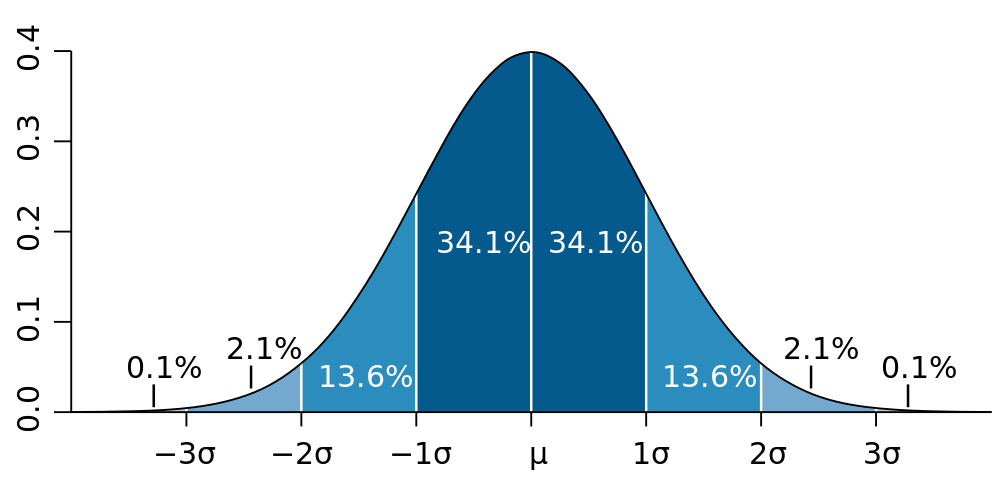
\includegraphics[width=\textwidth]{figures/bellcurve.png}
\caption[Standard normal distribution]{The curve from which the feature vectors are sampled. The vertical axis is the probability. The $\sigma$ values depict the standard deviations. \label{gaussianDistribution}}
\end{figure}

\section{Hardware \label{sec:hardware}}
This section describes the hardware which is used to run the tests. Docker provides an abstract interface which allows us to run the stack on a set of homogeneous resources. Nevertheless the hardware impacts the actual performance, therefore is it important to describe the hardware which is essential to repreduce the same numbers. To create an isolated environment which is not affected by other processes running on the physical hardware, a dedicated server has been assigned. Quintors' local Dell PowerEdge T620 development-server `Big-Willem' has been assigned for running the algorithm and for producing the results. Big-Willem has two Intel Xeon cpu's with six cores each supporting Hyper-threading, thus providing 24 logical cores in total. The main memory consists of 128 gigabytes in total. The virtual machine runs on 16 cores, has 64 gigabytes of memory assigned to it and is fully dedicated to running the software stack.

\section{Results \label{sec:results}}

First, the general execution time as a function of the input size is analyzed in Subsection \ref{subsec:executionTime}. Second, the impact on the execution time by adding additional workers to the Spark cluster is explored in Subsection \ref{subsec:parallelization}. This gives a good insight in the parallelizability of the algorithm. Finally, the stages of the algorithm are defined and insights are given regarding the execution time per stage in Subsection \ref{subsec:shuffle-behaviour}.

\subsection{Execution time \label{subsec:executionTime}}

The total execution time provides insight of the execution time of the algorithm with a fixed number of resources. The number of observations is doubled for each iteration starting from $500$ up to $64 000$. Every iteration is performed five times to obtain stable results. The execution time is given in seconds and is measured after the initialization of the Spark-cluster until the results of the distributed computation are returned to the driver.

\begin{figure}[ht!]
    \begin{center}
        % GNUPLOT: LaTeX picture with Postscript
\begingroup
  \makeatletter
  \providecommand\color[2][]{%
    \GenericError{(gnuplot) \space\space\space\@spaces}{%
      Package color not loaded in conjunction with
      terminal option `colourtext'%
    }{See the gnuplot documentation for explanation.%
    }{Either use 'blacktext' in gnuplot or load the package
      color.sty in LaTeX.}%
    \renewcommand\color[2][]{}%
  }%
  \providecommand\includegraphics[2][]{%
    \GenericError{(gnuplot) \space\space\space\@spaces}{%
      Package graphicx or graphics not loaded%
    }{See the gnuplot documentation for explanation.%
    }{The gnuplot epslatex terminal needs graphicx.sty or graphics.sty.}%
    \renewcommand\includegraphics[2][]{}%
  }%
  \providecommand\rotatebox[2]{#2}%
  \@ifundefined{ifGPcolor}{%
    \newif\ifGPcolor
    \GPcolortrue
  }{}%
  \@ifundefined{ifGPblacktext}{%
    \newif\ifGPblacktext
    \GPblacktexttrue
  }{}%
  % define a \g@addto@macro without @ in the name:
  \let\gplgaddtomacro\g@addto@macro
  % define empty templates for all commands taking text:
  \gdef\gplbacktext{}%
  \gdef\gplfronttext{}%
  \makeatother
  \ifGPblacktext
    % no textcolor at all
    \def\colorrgb#1{}%
    \def\colorgray#1{}%
  \else
    % gray or color?
    \ifGPcolor
      \def\colorrgb#1{\color[rgb]{#1}}%
      \def\colorgray#1{\color[gray]{#1}}%
      \expandafter\def\csname LTw\endcsname{\color{white}}%
      \expandafter\def\csname LTb\endcsname{\color{black}}%
      \expandafter\def\csname LTa\endcsname{\color{black}}%
      \expandafter\def\csname LT0\endcsname{\color[rgb]{1,0,0}}%
      \expandafter\def\csname LT1\endcsname{\color[rgb]{0,1,0}}%
      \expandafter\def\csname LT2\endcsname{\color[rgb]{0,0,1}}%
      \expandafter\def\csname LT3\endcsname{\color[rgb]{1,0,1}}%
      \expandafter\def\csname LT4\endcsname{\color[rgb]{0,1,1}}%
      \expandafter\def\csname LT5\endcsname{\color[rgb]{1,1,0}}%
      \expandafter\def\csname LT6\endcsname{\color[rgb]{0,0,0}}%
      \expandafter\def\csname LT7\endcsname{\color[rgb]{1,0.3,0}}%
      \expandafter\def\csname LT8\endcsname{\color[rgb]{0.5,0.5,0.5}}%
    \else
      % gray
      \def\colorrgb#1{\color{black}}%
      \def\colorgray#1{\color[gray]{#1}}%
      \expandafter\def\csname LTw\endcsname{\color{white}}%
      \expandafter\def\csname LTb\endcsname{\color{black}}%
      \expandafter\def\csname LTa\endcsname{\color{black}}%
      \expandafter\def\csname LT0\endcsname{\color{black}}%
      \expandafter\def\csname LT1\endcsname{\color{black}}%
      \expandafter\def\csname LT2\endcsname{\color{black}}%
      \expandafter\def\csname LT3\endcsname{\color{black}}%
      \expandafter\def\csname LT4\endcsname{\color{black}}%
      \expandafter\def\csname LT5\endcsname{\color{black}}%
      \expandafter\def\csname LT6\endcsname{\color{black}}%
      \expandafter\def\csname LT7\endcsname{\color{black}}%
      \expandafter\def\csname LT8\endcsname{\color{black}}%
    \fi
  \fi
    \setlength{\unitlength}{0.0500bp}%
    \ifx\gptboxheight\undefined%
      \newlength{\gptboxheight}%
      \newlength{\gptboxwidth}%
      \newsavebox{\gptboxtext}%
    \fi%
    \setlength{\fboxrule}{0.5pt}%
    \setlength{\fboxsep}{1pt}%
\begin{picture}(7200.00,5040.00)%
    \gplgaddtomacro\gplbacktext{%
      \csname LTb\endcsname%
      \put(1870,704){\makebox(0,0)[r]{\strut{}$32768$}}%
      \csname LTb\endcsname%
      \put(1870,1074){\makebox(0,0)[r]{\strut{}$65536$}}%
      \csname LTb\endcsname%
      \put(1870,1444){\makebox(0,0)[r]{\strut{}$131072$}}%
      \csname LTb\endcsname%
      \put(1870,1814){\makebox(0,0)[r]{\strut{}$262144$}}%
      \csname LTb\endcsname%
      \put(1870,2184){\makebox(0,0)[r]{\strut{}$524288$}}%
      \csname LTb\endcsname%
      \put(1870,2554){\makebox(0,0)[r]{\strut{}$1.04858\times10^{6}$}}%
      \csname LTb\endcsname%
      \put(1870,2925){\makebox(0,0)[r]{\strut{}$2.09715\times10^{6}$}}%
      \csname LTb\endcsname%
      \put(1870,3295){\makebox(0,0)[r]{\strut{}$4.1943\times10^{6}$}}%
      \csname LTb\endcsname%
      \put(1870,3665){\makebox(0,0)[r]{\strut{}$8.38861\times10^{6}$}}%
      \csname LTb\endcsname%
      \put(1870,4035){\makebox(0,0)[r]{\strut{}$1.67772\times10^{7}$}}%
      \csname LTb\endcsname%
      \put(1870,4405){\makebox(0,0)[r]{\strut{}$3.35544\times10^{7}$}}%
      \csname LTb\endcsname%
      \put(1870,4775){\makebox(0,0)[r]{\strut{}$6.71089\times10^{7}$}}%
      \csname LTb\endcsname%
      \put(2002,484){\makebox(0,0){\strut{}$256$}}%
      \csname LTb\endcsname%
      \put(2602,484){\makebox(0,0){\strut{}$512$}}%
      \csname LTb\endcsname%
      \put(3202,484){\makebox(0,0){\strut{}$1024$}}%
      \csname LTb\endcsname%
      \put(3802,484){\makebox(0,0){\strut{}$2048$}}%
      \csname LTb\endcsname%
      \put(4403,484){\makebox(0,0){\strut{}$4096$}}%
      \csname LTb\endcsname%
      \put(5003,484){\makebox(0,0){\strut{}$8192$}}%
      \csname LTb\endcsname%
      \put(5603,484){\makebox(0,0){\strut{}$16384$}}%
      \csname LTb\endcsname%
      \put(6203,484){\makebox(0,0){\strut{}$32768$}}%
      \csname LTb\endcsname%
      \put(6803,484){\makebox(0,0){\strut{}$65536$}}%
    }%
    \gplgaddtomacro\gplfronttext{%
      \csname LTb\endcsname%
      \put(176,2739){\rotatebox{-270}{\makebox(0,0){\strut{}Execution time in seconds}}}%
      \put(4402,154){\makebox(0,0){\strut{}Samples}}%
    }%
    \gplbacktext
    \put(0,0){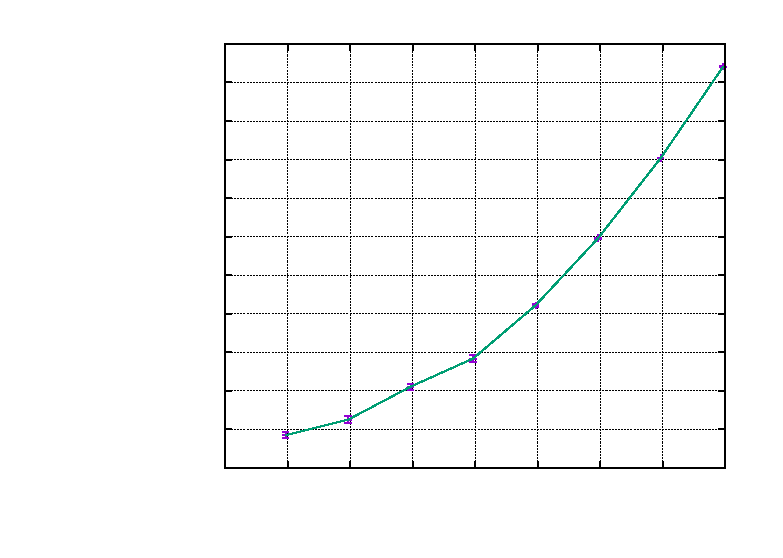
\includegraphics{plots/graph1}}%
    \gplfronttext
  \end{picture}%
\endgroup

    \caption{Execution time as a function of the input size.}
    \label{fig:executiontime}
    \end{center}
\end{figure}

In Figure \ref{fig:executiontime} we observe a quadratic increase in execution time, which is expected to be equal to the dominant computational complexity. In the case of the algorithm, the step of taking the Cartesian product for computing the distance matrix in Subsection \ref{subsec:distancematrix} is in order $\mathcal{O}(n^{2})$ and therefore the algorithm will perform analogous.

\subsection{Parallelization \label{subsec:parallelization}}

The purpose of this experiment is to determine the reduction of execution time by adding additional Spark workers to the cluster. Figure \ref{fig:parallelization} illustrates the execution time as a function of the number of workers.

A single Spark master and a single Apache Zookeeper instance is used. The number of Kafka nodes is equal to the number of Spark workers since when the number of workers increases, the number of partitions also needs to grow to parallelize the work and share the workload. Therefore more brokers are desirable to divide the partitions over different brokers. Each worker node within Apache Spark has 2 cores and 6 gigabytes of memory assigned.

\begin{figure}[ht!]
    \begin{center}
        % GNUPLOT: LaTeX picture with Postscript
\begingroup
  \makeatletter
  \providecommand\color[2][]{%
    \GenericError{(gnuplot) \space\space\space\@spaces}{%
      Package color not loaded in conjunction with
      terminal option `colourtext'%
    }{See the gnuplot documentation for explanation.%
    }{Either use 'blacktext' in gnuplot or load the package
      color.sty in LaTeX.}%
    \renewcommand\color[2][]{}%
  }%
  \providecommand\includegraphics[2][]{%
    \GenericError{(gnuplot) \space\space\space\@spaces}{%
      Package graphicx or graphics not loaded%
    }{See the gnuplot documentation for explanation.%
    }{The gnuplot epslatex terminal needs graphicx.sty or graphics.sty.}%
    \renewcommand\includegraphics[2][]{}%
  }%
  \providecommand\rotatebox[2]{#2}%
  \@ifundefined{ifGPcolor}{%
    \newif\ifGPcolor
    \GPcolortrue
  }{}%
  \@ifundefined{ifGPblacktext}{%
    \newif\ifGPblacktext
    \GPblacktexttrue
  }{}%
  % define a \g@addto@macro without @ in the name:
  \let\gplgaddtomacro\g@addto@macro
  % define empty templates for all commands taking text:
  \gdef\gplbacktext{}%
  \gdef\gplfronttext{}%
  \makeatother
  \ifGPblacktext
    % no textcolor at all
    \def\colorrgb#1{}%
    \def\colorgray#1{}%
  \else
    % gray or color?
    \ifGPcolor
      \def\colorrgb#1{\color[rgb]{#1}}%
      \def\colorgray#1{\color[gray]{#1}}%
      \expandafter\def\csname LTw\endcsname{\color{white}}%
      \expandafter\def\csname LTb\endcsname{\color{black}}%
      \expandafter\def\csname LTa\endcsname{\color{black}}%
      \expandafter\def\csname LT0\endcsname{\color[rgb]{1,0,0}}%
      \expandafter\def\csname LT1\endcsname{\color[rgb]{0,1,0}}%
      \expandafter\def\csname LT2\endcsname{\color[rgb]{0,0,1}}%
      \expandafter\def\csname LT3\endcsname{\color[rgb]{1,0,1}}%
      \expandafter\def\csname LT4\endcsname{\color[rgb]{0,1,1}}%
      \expandafter\def\csname LT5\endcsname{\color[rgb]{1,1,0}}%
      \expandafter\def\csname LT6\endcsname{\color[rgb]{0,0,0}}%
      \expandafter\def\csname LT7\endcsname{\color[rgb]{1,0.3,0}}%
      \expandafter\def\csname LT8\endcsname{\color[rgb]{0.5,0.5,0.5}}%
    \else
      % gray
      \def\colorrgb#1{\color{black}}%
      \def\colorgray#1{\color[gray]{#1}}%
      \expandafter\def\csname LTw\endcsname{\color{white}}%
      \expandafter\def\csname LTb\endcsname{\color{black}}%
      \expandafter\def\csname LTa\endcsname{\color{black}}%
      \expandafter\def\csname LT0\endcsname{\color{black}}%
      \expandafter\def\csname LT1\endcsname{\color{black}}%
      \expandafter\def\csname LT2\endcsname{\color{black}}%
      \expandafter\def\csname LT3\endcsname{\color{black}}%
      \expandafter\def\csname LT4\endcsname{\color{black}}%
      \expandafter\def\csname LT5\endcsname{\color{black}}%
      \expandafter\def\csname LT6\endcsname{\color{black}}%
      \expandafter\def\csname LT7\endcsname{\color{black}}%
      \expandafter\def\csname LT8\endcsname{\color{black}}%
    \fi
  \fi
    \setlength{\unitlength}{0.0500bp}%
    \ifx\gptboxheight\undefined%
      \newlength{\gptboxheight}%
      \newlength{\gptboxwidth}%
      \newsavebox{\gptboxtext}%
    \fi%
    \setlength{\fboxrule}{0.5pt}%
    \setlength{\fboxsep}{1pt}%
\begin{picture}(7200.00,5040.00)%
    \gplgaddtomacro\gplbacktext{%
      \csname LTb\endcsname%
      \put(1210,704){\makebox(0,0)[r]{\strut{}$65536$}}%
      \csname LTb\endcsname%
      \put(1210,2061){\makebox(0,0)[r]{\strut{}$131072$}}%
      \csname LTb\endcsname%
      \put(1210,3418){\makebox(0,0)[r]{\strut{}$262144$}}%
      \csname LTb\endcsname%
      \put(1210,4775){\makebox(0,0)[r]{\strut{}$524288$}}%
      \csname LTb\endcsname%
      \put(1342,484){\makebox(0,0){\strut{}$0$}}%
      \csname LTb\endcsname%
      \put(1888,484){\makebox(0,0){\strut{}$2$}}%
      \csname LTb\endcsname%
      \put(2434,484){\makebox(0,0){\strut{}$4$}}%
      \csname LTb\endcsname%
      \put(2980,484){\makebox(0,0){\strut{}$6$}}%
      \csname LTb\endcsname%
      \put(3526,484){\makebox(0,0){\strut{}$8$}}%
      \csname LTb\endcsname%
      \put(4073,484){\makebox(0,0){\strut{}$10$}}%
      \csname LTb\endcsname%
      \put(4619,484){\makebox(0,0){\strut{}$12$}}%
      \csname LTb\endcsname%
      \put(5165,484){\makebox(0,0){\strut{}$14$}}%
      \csname LTb\endcsname%
      \put(5711,484){\makebox(0,0){\strut{}$16$}}%
      \csname LTb\endcsname%
      \put(6257,484){\makebox(0,0){\strut{}$18$}}%
      \csname LTb\endcsname%
      \put(6803,484){\makebox(0,0){\strut{}$20$}}%
    }%
    \gplgaddtomacro\gplfronttext{%
      \csname LTb\endcsname%
      \put(176,2739){\rotatebox{-270}{\makebox(0,0){\strut{}Execution time in seconds}}}%
      \put(4072,154){\makebox(0,0){\strut{}Workers}}%
    }%
    \gplbacktext
    \put(0,0){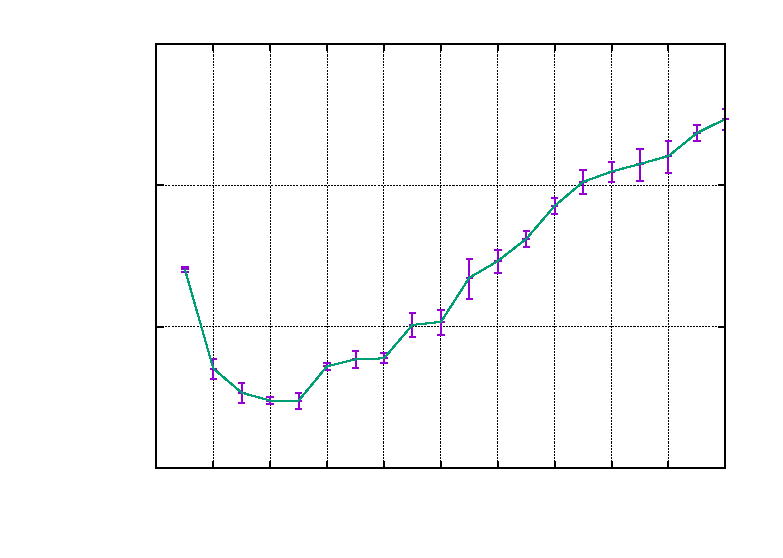
\includegraphics{plots/graph2}}%
    \gplfronttext
  \end{picture}%
\endgroup

        \caption[Execution time as a function of workers.]{Execution time as a function of the number of workers where each worker gets two cores and six gigabytes of RAM assigned, input size $n=2000$, and each worker has three partitions.}
        \label{fig:parallelization}
    \end{center}
\end{figure}

We observe that the execution time decreases until $\text{workers} = 5$, where the cluster works with 10 CPU's and 30 gigabytes of memory. For the relative small dataset of $n=2000$, the memory of each worker is not a resource constraint. The bottleneck is the processing power, which increases significantly when adding more nodes to the cluster. As the machine features 12 physical cores and 24 logical cores, the number of 10 CPU cores assigned to Spark is optimal, leaving some power for the Spark Master, Zookeeper and Apache Kafka instances. When increasing the number of nodes the context-switches are becoming dominant, therefore the number of nodes has to be chosen precisely according to the available hardware for obtaining the best resource utilization.

\subsection{Shuffle-behaviour \label{subsec:shuffle-behaviour}}

The shuffle-stages of Apache Spark are introduced in Subsection \ref{subsec_spark} and are known for having a major impact on the performance. Especially when the job is data-intensive in particular \cite{Chen:2009:UTI:1592681.1592693}. At a data-shuffle the RDD, which is scattered across different machines, re-distribution of the data from many to many machines is required. 

Even though moving data is expensive, sometimes it is necessary. For example, certain stages need to consolidate data on a single machine so that it can be co-located in memory to perform computations for the next stage. The algorithm contains two shuffle stages at:
\begin{description}
  \item[Distance matrix] At the first step, described in Subsection \ref{subsec:distancematrix}, the Cartesian product of the vector input is taken to construct the distance matrix between all pairs.
  \item[Outlier probabilities] The last step takes the product of the matrix, as described in Subsection \ref{subsec:outlierprobabilities}. As all the rows of the matrix are distributed across the different nodes. This requires a shuffle to transfer each row to a single machine to compute the final result. This stage does also includes the binary search to find the affinity for each row, as described in Subsection \ref{subsec:affinity}.
\end{description}

The Cartesian product is first computed using the \texttt{cartesian} primitive, which returns all the pairs of vectors. Then the \texttt{flatmap} primitive is used to compute the distances and leaves out the diagonal as it does not hold any information. Last, using \texttt{combineByKey} is used to reduce the pairs to a RDD of vectors which contain the distance from one to another observations. The intermediate steps, transforming the distance matrix to the affinity matrix in Subsection \ref{subsec:affinity} and computing the binding probability matrix as described in Subsection \ref{subsec:bindingprob} can be done locally on each worker for each vector in the RDD. Lastly, the position of the value in the vector is assigned a key and the final result is computed using \texttt{foldLeft} which requires a shuffle as the rows of the matrix are local, and the columns are distributed across multiple machines. Using the Spark Event Log\footnote{Spark monitoring \url{http://spark.apache.org/docs/latest/monitoring.html}}, the time taken for each stage can be monitored. This information is helpful to obtain insights about the bottlenecks of the algorithm.

\begin{table}[ht!]
\makebox[\linewidth]{
\centering

\begin{tabular}{r|llll|llll|llll}
 ~ & \multicolumn{4}{c|}{$N=2400$} & \multicolumn{4}{c|}{$N=4800$} & \multicolumn{4}{c}{$N=9600$}\\
 Stage & Distance & Product & Collect & Sum & Distance & Product & Collect & Sum & Distance & Product & Collect & Sum \\ \hline
 Run 1 & 114 & 90 & 6 & 210 & 258 & 330 & 6 & 594 & 900 & 1380 & 9 & 2289 \\
 Run 2 & 114 & 90 & 6 & 210 & 252 & 330 & 6 & 588 & 780 & 1380 & 12 & 2172 \\
 Run 3 & 114 & 90 & 6 & 210 & 258 & 330 & 6 & 594 & 900 & 1380 & 10 & 2290 \\
 Run 4 & 114 & 90 & 6 & 210 & 282 & 330 & 6 & 618 & 1080 & 1380 & 8 & 2468 \\
 Run 5 & 108 & 102 & 6 & 216 & 264 & 330 & 6 & 660 & 1260 & 1380 & 9 & 2649 \\
 Run 6 & 114 & 90 & 6 &	210 & 270 & 402 & 5 & 677 & 1080 & 1380 & 11 & 2471 \\
 Run 7 & 126 & 84 & 6 & 216 & 252 & 330 & 6 & 588 & 1320 & 1380 & 12 & 2712 \\
 Run 8 & 144 & 90 & 6 & 240 & 276 & 402 & 5 & 683 & 960 & 1380 & 12 & 2352 \\
 Run 9 & 138 & 102 & 6 & 246 & 270 & 330 & 5 & 605 & 900 & 1380 & 11 & 2291 \\
 Run 10 & 114 & 102 & 5 & 221 & 258 & 342 & 6 & 606 & 960 & 1380 & 11 & 2351 \\ \hline
 Average & 120.00 & 93.00 & 5.9 & 218.9 & 5.7 & 345.6 & 264 & 615.3 & 1014 & 1380 & 10.5 & 2404.5 \\
 Std.dev & 12.00 & 6.48 & 0.32 & 13.32 & 0.48 & 29.96 & 10.2 & 35.31 & 170.76 & 0 & 1.43 & 177.56 \\ \hline
 Total & 42.49\% & 54.82\% & 2.70\% & ~ & 42.91\% & 56.17\% & 0.92\% & ~ & 42.17\% & 57.39\% & 0.43\% & ~ \\
\end{tabular}
}
\caption[Execution time taken per stage]{Time taken for each stage of the algorithm execution. The distance column refers to the Cartesian product of the vectors to compute the distance-matrix. The product column refers to the shuffle required to consolidate each column of the matrix on a single worker. The collect column is the time taken to bring the results back to the driver. All numbers are in seconds.}

\label{table:executionPerStage}

\end{table}

Table \ref{table:executionPerStage} provides insights in the execution time per stage. Each stage is delimited by a shuffle at which the different worker nodes in the cluster have to coordinate and transfer the data which is required for the next stage. We observe that the last stage, which entails the binary search and the shuffling of the columns, covers the majority of the execution time. At first glance the Cartesian product is likely to be the dominant factor, but the share of this stage decreases as the number of observations grows.
